%% MACA: Experience-Compiled Multi-Agent Collision Avoidance
%% Compile: pdflatex maca.tex  (run twice for references)
\documentclass[conference]{IEEEtran}
\IEEEoverridecommandlockouts

\usepackage{cite}
\usepackage{amsmath,amssymb,amsfonts}
\usepackage{algorithm}
\usepackage{algorithmic}
\usepackage{graphicx}
\usepackage{textcomp}
\usepackage{xcolor}
\usepackage{booktabs}
\usepackage{tikz}
\usetikzlibrary{shapes.geometric,arrows.meta,positioning,calc,backgrounds,fit}

\def\BibTeX{{\rm B\kern-.05em{\sc i\kern-.025em b}\kern-.08em T\kern-.1667em\lower.7ex\hbox{E}\kern-.125emX}}

\begin{document}

\title{Experience-Compiled Multi-Agent Collision Avoidance:\\
Moving Large Language Models off the Real-Time Path\\
via Offline Law Discovery}

\author{
\IEEEauthorblockN{Shiyue Zhao}
\IEEEauthorblockA{\textit{Collision Avoidance Decision Systems}\\
shiyuez.umich@gmail.com}
}

\maketitle

\begin{abstract}
Large language models (LLMs) can arbitrate among extreme collision-avoidance
maneuvers---full braking, sharp lane changes, and T-type drift that presents
the vehicle's energy-absorbing rear to an unavoidable impact---by weighing
safety, legality, and structural crash mechanics. Yet a single LLM inference
costs seconds, while an extreme-avoidance decision window is often below
$300$\,ms. Prior work either accepts this latency or hides it behind
anticipatory background deliberation that still fails on first encounters.
We propose \textbf{MACA} (Multi-Agent Collision Avoidance), an
\emph{experience-compiled} architecture that removes the LLM from the
real-time path entirely. A multi-agent offline \emph{factory} discovers
decision \emph{laws} by designing parameterized scenario experiments,
sweeping them through a deterministic medium-fidelity dynamics simulator that
provides ground truth, inducing rules whose numeric boundaries are
cross-checked point-by-point against the sweep grid, and deliberating the
ambiguous residual into a case library. The \emph{online} plane executes this
compiled rule/case library by pure local matching---no LLM, no network---with
a measured trigger-path latency of $1$--$2$\,ms that is \emph{constant in
library size}, because the case-retrieval query is a locally computed numeric
feature vector rather than an API embedding. LLM spending is gated on
non-coverage; rule-versus-case conflicts are resolved online by deterministic
conservative arbitration and offline by adjudication, yielding a self-healing
library. Across nine calibrated scenarios spanning six maneuver classes, the
online plane selects the least-harm maneuver in every case with zero LLM
calls on the critical path, and an injected uncovered scene is shown to
close the online$\to$gap$\to$factory$\to$case self-healing loop end to end.
\end{abstract}

\begin{IEEEkeywords}
collision avoidance, autonomous driving, large language models, multi-agent
systems, real-time decision making, Hamilton-Jacobi reachability
\end{IEEEkeywords}

\section{Introduction}

Extreme collision-avoidance situations---a truck crossing laterally at an
intersection, cargo tumbling into the lane---demand, within a fraction of a
second, the selection of the least-harmful maneuver from a rich repertoire:
full emergency braking, sharp or braked lane changes, and, when a collision
is already unavoidable, a T-type drift that rotates the structurally strong,
energy-absorbing rear of the vehicle toward the incoming object rather than
its weak side (which, for electric vehicles, houses the battery). The
published SACA framework~\cite{saca} showed that a large language model (LLM)
can perform this arbitration by reasoning jointly over geometry, traffic
rules, and crash mechanics.

The obstacle is latency. A single LLM inference---even with a lightweight
model and thinking disabled---takes on the order of seconds to complete one
round of multi-agent negotiation, whereas the actionable window in an extreme
encounter is frequently under $300$\,ms. \emph{An LLM, however capable,
simply cannot answer in time.} An anticipatory design that deliberates in the
background during the risk build-up and caches a policy for the trigger
instant reduces the trigger-time cost to a table lookup, but the background
deliberation ($12$--$135$\,s in our measurements) routinely fails to finish
within the anticipation window, leaving first-encounter scenes unsafe.

We resolve this tension by \emph{never running the LLM online at all}. Our
key observation is that the value of the LLM is its \emph{reasoning}, and
reasoning can be \emph{compiled offline} into two artifacts that a
microsecond-to-millisecond matcher can execute: (i) \emph{rules}---empirical
laws with machine-checkable guards over a deterministic feature language and
a contingency policy-tree payload; and (ii) \emph{cases}---verified policies
for the regions where no clean law exists. This is the sense in which the
multi-agent system is a \emph{compiler} and the runtime executes its
\emph{compiled output}.

Our contributions are:
\begin{enumerate}
\item A \textbf{two-plane experience-compiled architecture} that amortizes
all LLM latency into an offline factory, so the online plane is LLM-free and
network-free, achieving a trigger-path latency of $1$--$2$\,ms that is
constant in library size.
\item A \textbf{grid-sweep law-discovery} process in which the LLM designs
parameterized experiments and induces laws, a deterministic simulator
supplies ground truth, and every induced rule boundary is
\emph{numerically cross-checked} against the sweep grid, so LLM
hallucinations are caught before a rule can be armed.
\item A \textbf{coverage-gated activation} policy: LLM tokens are spent only
on scenes the library does not already handle correctly, and a rule that
matches but is severity-suboptimal is treated as a counterexample that
refines the rule rather than as coverage.
\item A \textbf{conflict-driven self-healing} mechanism: online rule/case
disagreements are resolved by deterministic conservative arbitration (each
candidate is simulated and the lower-severity one executes) and queued for
offline adjudication that retires the losing entry.
\item A \textbf{medium-fidelity analytic dynamics simulator} (rectangular
oriented-bounding-box collision, friction-circle coupling, first-order
actuator lag with jerk limiting) realistic enough to expose that compromise
maneuvers such as braked lane changes are rarely strictly optimal, yet fast
enough (sub-millisecond per maneuver) to serve both the online arbiter and
the offline sweep. An optional CARLA backend is provided for offline
high-fidelity cross-validation.
\end{enumerate}

\section{Related Work}

\textbf{LLM-based driving decisions.} DiLu~\cite{dilu} and
SafeDrive~\cite{safedrive} use an LLM as a reasoning-and-reflection agent
over textual scene descriptions, accumulating experience in a memory module.
Agent-Driver~\cite{agentdriver} equips the LLM with a tool library.
DriveVLM~\cite{drivevlm} and dual-system designs such as
LeapAD~\cite{leapad} pair a slow LLM reasoner with a fast reactive
controller. In all of these the slow system remains \emph{on} the runtime
path; MACA differs by compiling the slow system entirely offline so that
nothing but a deterministic matcher runs online.

\textbf{Runtime assurance and reachability.} Hamilton--Jacobi (HJ)
reachability~\cite{hj} provides a value function over states that certifies
safety. We reuse a trained HJ value network as a \emph{state-risk reference}
---a reflex-layer monitoring signal and an end-state validation
constraint---rather than as the final arbiter, which is the simulated crash
severity.

\textbf{Scenario generation and falsification.} Search-based scenario
generation stresses a policy by optimizing for failures. Our generator
instead designs \emph{parameterized families} whose deterministic sweep
reveals \emph{where} a decision law holds, turning generation into experiment
design rather than adversarial search.

\section{Problem Formulation}

\subsection{Scene, maneuvers, and severity}
Let a \emph{scene} $s=(o_{-1},o_0)$ be an ordered pair of ego-centric
snapshots---a \emph{preview} frame $o_{-1}$ and a \emph{trigger} frame
$o_0$---each listing the ego state and a set of targets (vehicles, vulnerable
road users, obstacles) with position, velocity, type, and intention. The ego
selects a maneuver from the SACA repertoire
$\mathcal{A}=\{0,\dots,7\}$: $0$ full braking; $1,2$ sharp left/right lane
change; $3,4$ lane change with braking; $5,6$ T-drift nosing left/right; $7$
no intervention. A deterministic simulator $\Phi$ (Sec.~\ref{sec:sim}) maps a
scene and maneuver to a harm \emph{severity}
\begin{equation}
\sigma:\ \mathcal{S}\times\mathcal{A}\to\{0,1,2,3,4\},
\end{equation}
graded from no conflict ($0$) to severe injury likely ($4$). The ground-truth
least-harm action is
\begin{equation}
a^\star(s)\;=\;\arg\min_{a\in\mathcal{A}}\ \big(\sigma(s,a),\,e(s,a),\,\kappa(a)\big),
\label{eq:astar}
\end{equation}
ordered lexicographically by severity, then contact energy $e$, then maneuver
aggressiveness $\kappa$. Because rules and cases must react to how a scene
\emph{evolves}, the stored payload is not a scalar action but a
\emph{contingency policy tree} $\pi$: a map from a closed set of kinematic
evolution conditions $\mathcal{C}=\{$maintains, yields, accelerates,
secondary-activates, default$\}$ to actions, evaluated at the trigger instant
by comparing $o_{-1}$ and $o_0$.

\subsection{The latency constraint}
Let $\tau_{\mathrm{dec}}(s)$ be the actionable decision window and
$\ell(\cdot)$ the wall-clock latency of a decision procedure. An LLM
arbiter $\mathcal{M}$ realizes $a\approx a^\star$ but with
$\ell(\mathcal{M})\sim 10^0$--$10^1$\,s, whereas
$\tau_{\mathrm{dec}}(s)$ is frequently below $0.3$\,s, so
$\ell(\mathcal{M})\gg\tau_{\mathrm{dec}}$ and the arbiter is infeasible online.
The goal is a decision function $D$ with
\begin{equation}
\ell(D)\ll\tau_{\mathrm{dec}}
\quad\text{and}\quad
D(s)\approx a^\star(s)\ \text{on covered scenes,}
\end{equation}
\emph{and} $\ell(D)$ independent of the accumulated experience size---the
property that a naive case memory with an API-embedded query would violate.

\subsection{Two-plane decomposition}
We factor the arbiter into an offline \emph{compiler} $\mathcal{F}$ (the
multi-agent factory) and an online \emph{executor} $D$:
\begin{equation}
\mathcal{L}_{k+1}=\mathcal{F}(\mathcal{L}_k,\,Q_k),\qquad
a=D(s;\mathcal{L}),
\end{equation}
where $\mathcal{L}=(\mathcal{R},\mathcal{K})$ is the compiled library of rules
$\mathcal{R}$ and cases $\mathcal{K}$, and $Q_k$ is the feedback queue of
uncovered or conflicting scenes emitted by $D$. All LLM cost lives in
$\mathcal{F}$; $D$ is a pure, deterministic, network-free matcher. The
remainder of the paper specifies $D$ (Sec.~V), $\mathcal{F}$ (Sec.~VI), and
$\Phi,\sigma$ (Sec.~VII).

\section{Architecture Overview}

MACA separates \emph{thinking} from \emph{execution} into two planes
(Fig.~\ref{fig:arch}). The \textbf{online plane} runs on the vehicle in real
time and contains no LLM and no network dependency; it matches a compiled
rule/case library. The \textbf{offline factory} runs ahead of time, spends
LLM reasoning freely, and continually enriches the library. The two planes
share a single deterministic \emph{feature language} and a
\emph{kinematic/dynamic simulator}.

\begin{figure}[t]
\centering
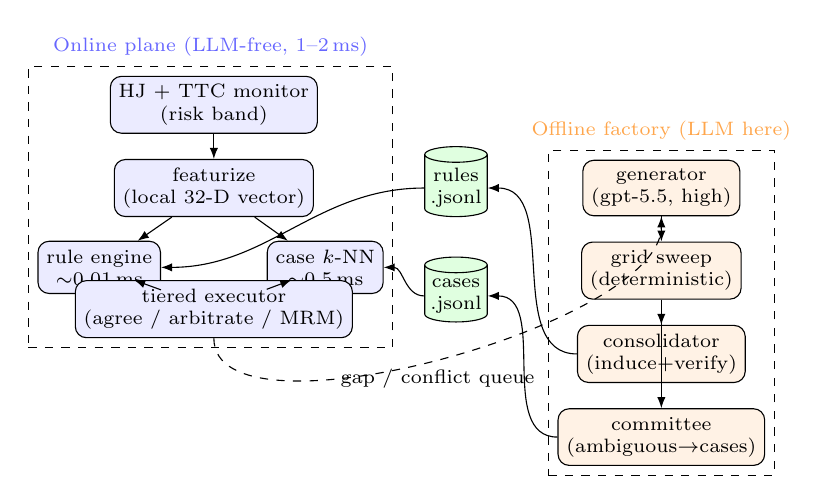
\begin{tikzpicture}[
  font=\scriptsize,
  box/.style={draw,rounded corners,align=center,inner sep=3pt,minimum height=6mm},
  online/.style={box,fill=blue!8},
  offline/.style={box,fill=orange!10},
  lib/.style={draw,cylinder,shape border rotate=90,aspect=0.25,fill=green!12,align=center,inner sep=2pt},
  arr/.style={-{Latex[length=1.4mm]}},
  node distance=3.2mm and 5mm
]
\node[online] (mon) {HJ + TTC monitor\\(risk band)};
\node[online,below=of mon] (feat) {featurize\\(local 32-D vector)};
\node[online,below left=3mm and -6mm of feat] (rule) {rule engine\\$\sim$0.01\,ms};
\node[online,below right=3mm and -6mm of feat] (case) {case $k$-NN\\$\sim$0.5\,ms};
\node[online,below=8mm of feat] (exec) {tiered executor\\(agree / arbitrate / MRM)};
\draw[arr] (mon)--(feat);
\draw[arr] (feat)--(rule);
\draw[arr] (feat)--(case);
\draw[arr] (rule)--(exec);
\draw[arr] (case)--(exec);
\node[lib,right=14mm of feat] (rules) {rules\\.jsonl};
\node[lib,below=5mm of rules] (cases) {cases\\.jsonl};
\draw[arr] (rules.west) to[out=180,in=0] (rule.east);
\draw[arr] (cases.west) to[out=180,in=0] (case.east);
\node[offline,right=12mm of rules] (gen) {generator\\(gpt-5.5, high)};
\node[offline,below=of gen] (sweep) {grid sweep\\(deterministic)};
\node[offline,below=of sweep] (cons) {consolidator\\(induce+verify)};
\node[offline,below=of cons] (comm) {committee\\(ambiguous$\to$cases)};
\draw[arr] (gen)--(sweep);
\draw[arr] (sweep)--(cons);
\draw[arr] (sweep)--(comm);
\draw[arr] (cons.west) to[out=180,in=0] (rules.east);
\draw[arr] (comm.west) to[out=180,in=0] (cases.east);
\draw[arr,dashed] (exec.south) to[out=-90,in=-90,looseness=0.6] node[below,pos=0.5]{gap / conflict queue} (gen.south);
\begin{scope}[on background layer]
\node[draw,dashed,fit=(mon)(feat)(rule)(case)(exec),label={[blue!60]above:Online plane (LLM-free, $1$--$2$\,ms)}] {};
\node[draw,dashed,fit=(gen)(sweep)(cons)(comm),label={[orange!70]above:Offline factory (LLM here)}] {};
\end{scope}
\end{tikzpicture}
\caption{Two-plane experience-compiled architecture. The offline factory
discovers laws and compiles them into a rule/case library; the online plane
executes the library by pure local matching. Uncovered scenes and rule/case
conflicts flow back to the factory.}
\label{fig:arch}
\end{figure}

The maneuver repertoire follows SACA: code $0$ full braking; $1$/$2$ sharp
left/right lane change; $3$/$4$ lane change with braking; $5$/$6$ T-drift
with the nose pointing left/right (rear meets the threat); $7$ no
intervention. Rules and cases do not carry a single action but a
\emph{contingency policy tree} whose branches are guarded by a closed set of
kinematic evolution conditions (threat maintains / yields / accelerates /
secondary activates / default), so that at the trigger instant the reflex
loop classifies how the scene actually evolved between two snapshots and
selects the matching branch in microseconds without parsing free text.

\section{Online Plane}

\subsection{Feature language and reflex monitor}
A deterministic feature map $\phi:\mathcal{S}\to\mathbb{R}^{32}$ encodes every
scene \emph{locally}---no API embedding. It concatenates eight normalized
numeric features clipped to $[0,1]$ (TTC, predicted miss distance, lateral
distance and speed, closing speed, ego speed, HJ risk, threat distance) with
one-hot encodings of the discrete features: an eight-way approach sector
($8$), pedestrian side ($3$), road topology ($3$), threat kind ($6$), and four
booleans (left/right corridor free, a simulation-grounded
\texttt{braking\_sufficient} flag, an on-collision-course flag):
\begin{equation}
\phi(s)=\big[\underbrace{\hat n_1\!\cdots\hat n_8}_{8},\ \underbrace{\mathbf{1}_{\mathrm{sect}}}_{8},\ \underbrace{\mathbf{1}_{\mathrm{ped}}}_{3},\ \underbrace{\mathbf{1}_{\mathrm{topo}}}_{3},\ \underbrace{\mathbf{1}_{\mathrm{kind}}}_{6},\ \underbrace{b_1{:}b_4}_{4}\big].
\end{equation}
This construction is the crux of the constant-latency property: the query
vector is computed in $\mu$s from scene geometry, so retrieval never touches
the network. The reflex monitor combines HJ state risk and TTC urgency,
\begin{equation}
\rho \;=\; 0.6\,\rho_{\mathrm{HJ}} \;+\; 0.4\,\max\!\Big(0,\,1-\tfrac{\mathrm{TTC}}{3\,\mathrm{s}}\Big),
\end{equation}
and bands the scene as low ($\rho<0.40$), elevated ($<0.63$), or critical.
The plane \emph{commits} when the band is critical, or when the threat is on a
collision course that braking can no longer resolve
($\texttt{braking\_sufficient}=\text{false}$, itself decided by simulating
code $0$ and testing $\sigma(s,0)\le1$)---``cannot brake out of it'' is a
commit point even below the critical threshold.

\subsection{Rule and case matching}
A rule $r=(g_r,\pi_r)$ carries guards $g_r$ over any subset of the feature
language and \emph{matches} $s$ iff every discrete guard admits $\phi(s)$'s
value and every numeric guard's interval contains it:
\begin{equation}
\mathrm{match}(r,s)\!\iff\!\!\bigwedge_{k\in\mathrm{disc}}\!\! v_k(s)\!\in\! g_r^k \;\wedge\!\!\bigwedge_{k\in\mathrm{num}}\!\! v_k(s)\!\in\![g_r^{k,\downarrow},g_r^{k,\uparrow}].
\end{equation}
The schema is open-ended: a new feature becomes matchable without touching the
engine. Matching sorts candidates by specificity ($|g_r|$), then priority,
then validated pass rate, at $\sim$0.01\,ms. Cases are retrieved by cosine
$k$-NN ($k{=}3$) over the locally built vector,
\begin{equation}
c^\star=\arg\max_{c\in\mathcal{K}}\frac{\langle\phi(s),\phi(c)\rangle}{\lVert\phi(s)\rVert\,\lVert\phi(c)\rVert},\quad
\text{hit iff }\cos\ge\tau\,(=0.92),
\end{equation}
which is a single \texttt{numpy} matrix--vector product---$\sim$1\,ms at
$10^3$ cases, $\sim$10\,ms at $10^5$, and $O(\log|\mathcal{K}|)$ with an HNSW
index. \textbf{Library growth therefore does not threaten real time}; latency
is guaranteed by construction, not by capping library size.

\subsection{Tiered execution and conservative arbitration}
The executor is tiered (Alg.~\ref{alg:online}). If a rule and a case agree,
execute. If they disagree on the maneuver, resolve by \emph{conservative
arbitration}: simulate both candidates and execute
\begin{equation}
a=\arg\min_{a'\in\{a_r,a_c\}}\big(\sigma(s,a'),\,e(s,a'),\,\kappa(a')\big),
\end{equation}
in $\sim$0.1\,ms, and queue the conflict for offline adjudication (unless the
winning case is itself a settled adjudication). If only one side hits, take
it; if neither does, execute the minimal-risk maneuver (full braking) and
queue the scene as a gap. Control authority is never suspended.

\begin{algorithm}[t]
\caption{Online decision $D(s;\mathcal{L})$ (LLM-free)}
\label{alg:online}
\begin{algorithmic}[1]
\STATE $\rho,\text{band}\leftarrow\textsc{Monitor}(s)$
\IF{band $=$ low \textbf{and} braking resolves}
  \RETURN $7$ \COMMENT{no intervention}
\ENDIF
\STATE $x\leftarrow\phi(s)$;\quad $c\leftarrow\textsc{EvolutionClass}(o_{-1},o_0)$
\STATE $r\leftarrow\textsc{RuleMatch}(x)$;\quad $k\leftarrow\textsc{CaseKNN}(x)$
\STATE $a_r\leftarrow\pi_r[c]$;\quad $a_c\leftarrow\pi_k[c]$
\IF{$r$ and $k$ hit and $a_r\ne a_c$}
  \STATE $a\leftarrow\arg\min_{a'\in\{a_r,a_c\}}(\sigma,e,\kappa)$;\ \ \textsc{Queue}(conflict)
\ELSIF{$r$ or $k$ hits}
  \STATE $a\leftarrow$ the hitting side
\ELSE
  \STATE $a\leftarrow 0$;\quad \textsc{Queue}(gap) \COMMENT{minimal-risk fallback}
\ENDIF
\RETURN $a$
\end{algorithmic}
\end{algorithm}

\subsection{Latency}
Table~\ref{tab:latency} reports the per-stage trigger-path budget measured on
the demo scenarios. The total is $1$--$2$\,ms (warm), with zero LLM calls and
zero network I/O; the first invocation adds a one-time $\sim$15\,ms of
PyTorch initialization for the HJ network.

\begin{table}[t]
\caption{Measured trigger-path latency budget (warm).}
\label{tab:latency}
\centering
\begin{tabular}{@{}lll@{}}
\toprule
Stage & Module & Latency \\
\midrule
Reflex risk monitor & \texttt{monitor} & $\sim$1\,ms \\
Featurization & \texttt{features} & $\sim$0.3\,ms \\
Rule matching & \texttt{rule\_engine} & $\sim$0.01\,ms \\
Case $k$-NN & \texttt{case\_index} & $\sim$0.05--0.5\,ms \\
Evolution classification & \texttt{policy\_match} & $\sim$0.1\,ms \\
Conservative arbitration (if conflict) & \texttt{arbiter} & $\sim$0.1\,ms \\
\midrule
\textbf{Trigger-path total} & \texttt{executor} & \textbf{$\mathbf{1}$--$\mathbf{2}$\,ms} \\
\bottomrule
\end{tabular}
\end{table}

\section{Offline Factory}

The factory (Fig.~\ref{fig:arch}, right) enriches the library in batches
(Alg.~\ref{alg:factory}). A scene is \emph{covered} when an active rule matches
it with a severity-optimal maneuver or a case exceeds the similarity
threshold; the predicate
\begin{equation}
\mathrm{cov}(s)\!=\!\big(\exists r{:}\,\mathrm{match}(r,s)\wedge \pi_r\!=\!a^\star(s)\big)\vee\big(\exists c{:}\cos(\phi(s),\phi(c))\!\ge\!\tau\big)
\end{equation}
gates every LLM call, so tokens are spent only where the library is wrong.

\begin{algorithm}[t]
\caption{Factory batch $\mathcal{F}(\mathcal{L},Q)$ (LLM offline)}
\label{alg:factory}
\begin{algorithmic}[1]
\STATE \textbf{Phase 1 — drain feedback queue $Q$:}
\FORALL{$s\in Q$}
  \IF{$\mathrm{cov}(s)$ \textbf{or} $s$ is doomed}
    \STATE \textbf{continue} \COMMENT{skip; no token, no meaningless case}
  \ENDIF
  \STATE $\mathcal{K}\!\leftarrow\!\mathcal{K}\cup\textsc{Committee}(s)$; if conflict, retire loser
\ENDFOR
\STATE \textbf{Phase 2 — discover laws:}
\FOR{$n$ families}
  \STATE $\mathcal{G}\leftarrow$ \textsc{Generator}(coverage briefing)
  \STATE grid $\leftarrow$ \textsc{Sweep}$(\mathcal{G})$; label each point lawful/ambiguous/doomed
  \STATE $P^{\mathrm{law}}\!\leftarrow\{$uncovered lawful$\}$; counterexamples $\leftarrow\{$rule-suboptimal$\}$
  \FORALL{rule $\hat r\in$ \textsc{Consolidate}$(P^{\mathrm{law}},\text{counterex.})$}
    \IF{\textsc{NumericCrossCheck}$(\hat r,\text{grid})$ \textbf{and} \textsc{Battery}$(\hat r)\!\ge\!0.9$}
      \STATE arm $\hat r$ as \texttt{active}
    \ENDIF
  \ENDFOR
  \STATE $\mathcal{K}\leftarrow\mathcal{K}\cup\{\textsc{Committee}(p):p\in\text{uncovered ambiguous}\}$
\ENDFOR
\STATE \textbf{Phase 3:} re-validate a sample of active rules; deprecate stale
\RETURN $\mathcal{L}$
\end{algorithmic}
\end{algorithm}

\subsection{Experiment design and grid sweep}
A generator agent (a high-reasoning LLM) designs a \emph{parameterized
scenario family}: a pattern (lateral crossing, lead braking, cut-in, static
blockage), a context template (topology, threat type, pedestrian side, road
boundaries, blocked corridor, follower), and swept parameter ranges. The LLM
never emits raw coordinates; instantiation is deterministic and places
threats on a collision course by construction, so physical plausibility is
guaranteed. Each grid point then simulates all eight maneuvers and ranks them
by severity. Points where one maneuver dominates by at least one severity
class, or where a mild action fully resolves the scene, are \emph{lawful};
harmful near-ties and points whose best option still injures a vulnerable
road user are \emph{ambiguous}; points where every maneuver is maximally
severe with no discrimination are \emph{doomed} and discarded.

\subsection{Law induction with numeric cross-check}
A consolidator agent (a medium-reasoning LLM) induces general rules from the
lawful region. Every proposal is verified \emph{point-by-point} against the
sweep grid: for each grid point matching the proposed guards, the branch's
maneuver must actually achieve that point's minimum severity, and at least
three points must be covered. Unsupported boundaries are rejected back to the
LLM with the specific mismatches, up to two rounds. This numeric gate is what
lets the system \emph{use} the LLM's generalization while refusing to
\emph{trust} it: a hallucinated boundary cannot survive.

\subsection{Promotion, ambiguity, and anti-drift}
A candidate rule is promoted to \texttt{active} only after passing a
regression battery (its source grid plus static regression scenarios plus
pedestrian-side/boundary/HJ constraints) at $\ge$90\%. Ambiguous points are
sent to a committee (decision + consistency-gated debate + a deterministic
safety layer with a veto/re-decide loop) that produces cases carrying a
lesson. Every batch re-validates a sample of active rules against their
re-instantiated source families; a rule that no longer holds---for example
after the simulator is upgraded---is automatically deprecated. Turning
simulator evolution into automatic library maintenance is a feature, not a
failure mode.

\subsection{Coverage-gated activation}
Every LLM call is gated on \emph{non-coverage}: a scene or grid point is
covered when an active rule matches it with a severity-optimal maneuver, or a
case above the similarity threshold does. Covered queue items are skipped,
consolidation is skipped when the lawful region is already ruled, and
committee time goes only to uncovered ambiguous points. Critically, a rule
that \emph{matches but is severity-suboptimal} is not coverage---it is a
\emph{counterexample} fed back to the consolidator, which is how an imperfect
seed domain rule (e.g.\ a T-drift rule that over-claims a region where a
clean escape exists) is corrected by evidence.

\section{Medium-Fidelity Dynamics Simulator}
\label{sec:sim}

Both planes rely on a deterministic simulator $\Phi$ as ground truth, so it
must be realistic yet sub-millisecond. The ego is a rectangle; the horizon is
$H{=}2.5$\,s at step $\Delta t{=}0.05$\,s. Three ingredients lift it above a
point-mass-and-circle model while keeping it analytic.

\subsection{Ego rollout}
Each maneuver defines a world-frame acceleration command
$a^{\mathrm{cmd}}(\cdot)$ and a target heading. The command passes through a
first-order \textbf{actuator lag} with a \textbf{jerk} ceiling,
\begin{equation}
\tilde a_{k+1}=a_k+\big(a^{\mathrm{cmd}}_k-a_k\big)\tfrac{\Delta t}{\varsigma+\Delta t},\quad
a_{k+1}=a_k+\mathrm{clip}\big(\tilde a_{k+1}-a_k,\,J\Delta t\big),
\end{equation}
with $\varsigma{=}0.12$\,s, $J{=}40$\,m/s$^3$, and then a
\textbf{friction-circle} projection: for ordinary maneuvers ($0$--$4$) the
combined acceleration obeys $\lVert a\rVert\le\mu g$ ($\mu{=}0.9$), so a
vehicle cannot brake and steer at full authority at once; T-drift ($5$/$6$) is
a deliberate slip maneuver with a higher slip cap $a_{\max}^{\mathrm{drift}}$.
States integrate as $v_{k+1}=\max(0,v_k+a_{k+1}\Delta t)$, $p_{k+1}=p_k+v_{k+1}\Delta t$.

\subsection{Oriented bounding-box contact}
Targets are circles of type-dependent radius $r$; the ego is an
$L{\times}W$ box with heading $\theta$. Transforming a target center into the
body frame, $(l_x,l_y)=R(-\theta)(c-p)$, the signed gap and impact face are
\begin{equation}
g=\big\lVert(\max(|l_x|-\tfrac{L}{2},0),\ \max(|l_y|-\tfrac{W}{2},0))\big\rVert-r,
\end{equation}
\begin{equation}
\mathrm{face}=\begin{cases}\text{front/rear},&|l_x|/\tfrac{L}{2}\ge|l_y|/\tfrac{W}{2}\\\text{side},&\text{otherwise,}\end{cases}
\end{equation}
so the impact face \emph{rotates with heading}. This is what makes T-drift
work: as the body swings toward $\theta\!\approx\!90^\circ$, a laterally
incoming threat meets the rear rather than the flank.

\subsection{Two-phase T-drift}
The drift is modeled in two phases. During rotation ($t<T_{\mathrm{rot}}\!\approx\!0.9$\,s)
the heading ramps to $\pm90^\circ$ under a longitudinal brake plus a lateral
kick that builds the slide. Once perpendicular, the tires are saturated and
the maneuver becomes a \emph{skid}: friction decelerates the velocity
\emph{vector} to rest,
$a^{\mathrm{cmd}}=-a_{\max}^{\mathrm{drift}}\,v/\lVert v\rVert$,
rather than continuing to accelerate sideways. This yields a bounded, physical
trajectory (the car stops rotated, having slid a few metres) instead of an
unbounded lateral run-off, while leaving the early impact-phase geometry---and
thus the crash outcome---unchanged.

\subsection{Severity}
Severity grades contact relative speed $v_{\mathrm{rel}}$ and adjusts for
structure and vulnerability:
\begin{equation}
\sigma=\mathrm{clip}\Big(\underbrace{\beta(v_{\mathrm{rel}})}_{2/3/4}+\underbrace{\delta_{\mathrm{face}}}_{-1\,\mathrm{rear},\,+1\,\mathrm{side}}+\underbrace{2\cdot\mathbb{1}_{\mathrm{VRU}}}_{}\ ,\,2,\,4\Big),
\end{equation}
with $\beta{=}2/3/4$ for $v_{\mathrm{rel}}<3/<8/\ge8$\,m/s, no-contact scenes
scoring $0$ (or $1$ for a sub-$0.5$\,m near miss), and road-boundary
departures counted as side barrier collisions. The rear bonus and side penalty
encode that energy-absorbing structure sits fore/aft while the flanks---and,
for EVs, the battery---are weak. A pluggable backend admits an optional
high-fidelity CARLA backend for offline cross-validation; being second-scale
it never enters the online or sweep hot path.

A notable consequence of the realistic dynamics is that
lane-change-with-braking (codes $3$/$4$) is \emph{rarely strictly optimal} in
any single scene: it is a compromise dominated by either pure braking or a
pure lane change. This is a faithful physical finding, and the architecture
accommodates it---codes $3$/$4$ survive as conditional policy-tree branches
rather than as standalone rules.

\section{Experiments}

\subsection{Setup}
We evaluate on nine calibrated scenarios spanning six maneuver classes
(Table~\ref{tab:scen}), each stressing a different online tier. Factory
agents use a high-reasoning model for generation, a medium-reasoning model
for induction, and lightweight no/low-reasoning models for the committee; the
online plane uses no model. All timings are on a commodity laptop CPU; the
online plane runs with the API key unset to confirm network independence.

\begin{table}[t]
\caption{Demo scenarios and the online tier each exercises.}
\label{tab:scen}
\centering
\begin{tabular}{@{}llp{3.2cm}@{}}
\toprule
Scenario & Best & Online path \\
\midrule
\texttt{test1} & 6 & seed T-drift rule + case (rear impact) \\
\texttt{cross\_right\_tdrift} & 5 & seed T-drift rule (mirror) \\
\texttt{cross\_escape} & 2 & case overrides over-broad rule via arbitration \\
\texttt{moving\_obstacle} & 1 & case (moving obstacle, boundary) \\
\texttt{test2} & 0 & braking-sufficient rule \\
\texttt{cut\_in\_brake} & 0 & braking-sufficient rule \\
\texttt{highway\_brake} & 0 & case \\
\texttt{blockage\_left\_escape} & 0 & MRM fallback (commit condition) \\
\texttt{low\_risk} & 7 & reflex pass-through \\
\bottomrule
\end{tabular}
\end{table}

\subsection{Online decision correctness and latency}
On all nine scenarios the online plane selects the maneuver that the
simulator ranks least-harmful ($9/9$), with a trigger-path latency of
$1$--$2$\,ms (measured maximum $1.53$\,ms) and zero LLM/network activity.
Repeated runs are stable and the feedback queue remains empty once the
library is consistent. Table~\ref{tab:sevmatrix} makes the least-harm
selection legible: in each row exactly the executed maneuver attains the
minimum severity while the alternatives are strictly worse.

\begin{table}[t]
\caption{Simulated severity of each maneuver (0=safe\,$\dots$\,4=severe) on
representative scenes; \textbf{bold} is the executed code. The chosen maneuver
is uniquely least-harm in every row.}
\label{tab:sevmatrix}
\centering\footnotesize
\setlength{\tabcolsep}{3.4pt}
\begin{tabular}{@{}lccccccccc@{}}
\toprule
Scene & 0 & 1 & 2 & 3 & 4 & 5 & 6 & 7 & best\\
\midrule
\texttt{test1} & 4 & 4 & 4 & 4 & 4 & 4 & 3 & 4 & \textbf{6}\\
\texttt{cross\_escape} & 4 & 4 & 1 & 4 & 4 & 4 & 4 & 4 & \textbf{2}\\
\texttt{blockage\_left} & 3 & 4 & 4 & 4 & 4 & 4 & 4 & 4 & \textbf{0}\\
\texttt{highway\_brake} & 3 & 3 & 3 & 3 & 3 & 4 & 4 & 3 & \textbf{0}\\
\texttt{vru\_right\_block} & 4 & 4 & 1 & 4 & 4 & 4 & 3 & 4 & \textbf{2}\\
\bottomrule
\end{tabular}
\end{table}

The T-drift rows confirm the intended crash mechanism: in \texttt{test1} only
the rear-facing drift (code $6$) converts an otherwise severity-$4$ side
impact into a survivable severity-$3$ rear impact---every other maneuver,
including doing nothing, is struck on the flank at $\ge8$\,m/s. The
\texttt{vru\_right\_block} row is subtler: it is \texttt{test1} geometry with a
pedestrian standing on the drift-escape side, so the drift (still severity
$3$) is \emph{not} chosen---a clean lateral escape (code $2$, severity $1$)
threads past both truck and pedestrian and dominates.

\subsection{Consistency and self-healing}
The compiled library holds three domain seed rules and thirteen cases (eight
calibrated seeds plus five grown by the factory: three from committee
deliberation of ambiguous sweep points and two from queued runtime gaps). Two
interlock mechanisms are verified end to end. First, \emph{conflict-driven
correction}: in \texttt{cross\_escape} the over-broad seed T-drift rule (code
$6$) and a learned escape case (code $2$) disagree; conservative arbitration
simulates both and executes the lower-severity escape, and the conflict, once
adjudicated, does not recur. Second, \emph{self-healing coverage}: injected
VRU-trade-off scenes---a crossing truck whose usual T-drift is blocked by a
pedestrian on the escape side---match no rule, so the plane falls back to
minimal-risk braking and queues them; one offline batch deliberates each into
a case whose recommendation we independently verify to be the simulator's
least-harm action, after which the same scene (and, by $k$-NN generalization,
a nearby untrained variant) is decided by that case. A companion safeguard
mirrors the sweep's \emph{doomed}-point filter on the queue: a gap in which
every maneuver is maximally severe teaches nothing and is dropped rather than
compiled into a misleading ``recommend maneuver $X$'' case.

\subsection{Ablations (qualitative)}
Removing the numeric cross-check admits hallucinated rule boundaries that fail
the promotion battery. Removing coverage gating causes the factory to
re-deliberate already-covered regions, wasting tokens with no library growth.
Replacing the local feature vector with an API embedding reintroduces network
latency on the case-retrieval path, breaking the constant-latency property.

\section{Discussion and Limitations}

The realistic dynamics narrow the T-drift ``sweet spot'': if TTC is long
enough for the drift to complete its rotation, braking often also avoids the
collision, whereas if TTC is short, no maneuver completes in time. T-drift
remains optimal only in a band where a collision is unavoidable yet the
$\sim$1\,s rotation can still present the rear---consistent with the domain
rule's TTC~$\le 1.3$\,s precondition. Codes $3$/$4$ being rarely strictly
optimal is a genuine physical result rather than a modeling gap.

A concrete limitation surfaced by our own fault-injection is that a seed
domain rule keyed on the primary threat does not, by itself, consult the
escape corridor for \emph{secondary} occupancy: a T-drift rule can fire toward
a side already occupied by another vehicle. The architecture's designed remedy
is exactly the coverage-gated feedback loop---such a scene is a rule
counterexample that a sweep with a blocked-corridor template turns into a
tightened guard or an overriding case---but until that batch runs, online
conservative arbitration is the only backstop, so seeding rules with
corridor-aware guards is preferable. Finally, cases inherit the feature
encoding at creation time; changing the encoding requires re-coverage,
currently handled by the passive gap$\to$rebuild loop rather than an active
re-encoding pass.

\section{Conclusion}

MACA shows that the latency gap between LLM inference and real-time collision
avoidance can be closed not by making the LLM faster but by removing it from
the runtime entirely: a multi-agent offline factory compiles reasoning into a
rule/case library that a millisecond matcher executes, with law discovery
disciplined by a deterministic simulator and numeric cross-checking, LLM
spending gated on non-coverage, and conflicts healed automatically. The
online plane is LLM-free, network-free, and constant-latency in library size.

\begin{thebibliography}{00}
\bibitem{saca} S.~Zhao \emph{et al.}, ``Scenario-Aware Collision Avoidance
via Predictive Risk Assessment and LLM Reasoning,'' \emph{arXiv:2504.00115},
2025.
\bibitem{dilu} L.~Wen \emph{et al.}, ``DiLu: A Knowledge-Driven Approach to
Autonomous Driving with Large Language Models,'' in \emph{ICLR}, 2024.
\bibitem{safedrive} Z.~Zhou \emph{et al.}, ``SafeDrive: A Knowledge- and
Data-Driven Risk-Sensitive Decision-Making Framework for Autonomous
Vehicles,'' \emph{arXiv preprint}, 2024.
\bibitem{agentdriver} J.~Mao \emph{et al.}, ``A Language Agent for Autonomous
Driving,'' in \emph{COLM}, 2024.
\bibitem{drivevlm} X.~Tian \emph{et al.}, ``DriveVLM: The Convergence of
Autonomous Driving and Large Vision-Language Models,'' in \emph{CoRL}, 2024.
\bibitem{leapad} J.~Mei \emph{et al.}, ``Continuously Learning, Adapting, and
Improving: A Dual-Process Approach to Autonomous Driving,'' in
\emph{NeurIPS}, 2024.
\bibitem{hj} S.~Bansal \emph{et al.}, ``Hamilton--Jacobi Reachability: A Brief
Overview and Recent Advances,'' in \emph{IEEE CDC}, 2017.
\end{thebibliography}

\end{document}
